% ****************************************************************************************************
\chapter{Causal Loop Diagram -- A qualitative Model}\label{ch:cld}
% ****************************************************************************************************

\begin{flushright}{\slshape    
	We shape our buildings; thereafter, our buildings shape us.} \\ \medskip
	--- Winston Churchill
\end{flushright}

Within this chapter the essential interdependencies -- high-leverage interventions and policies -- between the previous described classification criteria respectively characteristics are reveled and illustrated using the concept of system dynamics, more specifically by means of a \ac{CLD} and thereby also answering the \thref{srq2}. System dynamics is an approach to study complexity and was originally developed at the \ac{MIT} by Jay W. \citet{Forrester1961}. John D. \citeauthor{Sterman2000} applied system dynamics to business and organizational problems -- a comprehensive \citep{Sterman2000} as well as brief \citep{Sterman2001} introductory guide is provided. Within this thesis the notation and guidelines provided by John D. \citeauthor{Sterman2000} are used (please refer to the above mentioned sources). The ulterior motive behind a \ac{CLD} is the simplification of reality by defining suitable model boundaries. \acp{CLD} \textit{"can never be comprehensive (and you shouldn't try: modeling is the art of simplification). They are also never final, but always provisional"} \citep[p. 166]{Sterman2000}. An important aspect of causal relationships within \acp{CLD} which should always bear in mind, is that the causal relations are modeled ceteris paribus (literally translated as 'with other things the same' or 'all other things being equal or held constant') \footnote{\textit{"A positive link means that if the cause increases, the effect increases above what it would otherwise have been, and if the cause decreases, the effect decreases below what it would otherwise have been. \ldots A negative link means that if the cause increases, the effect decreases below what it would otherwise have been, and if the cause decreases, the effect increases above what it would otherwise have been"} \citep[p. 139]{Sterman2000}.}.

In the beginning of this chapter the causal relationships for the generic customer segment in the \ac{PaaS} domain are discussed in Section \ref{ch:cld:cs}. Thereafter, interdependencies between the five identified customer segments are presented in Section \ref{ch:cld:csi}. At the end of this chapter the overall \ac{CLD} is depicted and explained in Section \ref{ch:cld:bp}.

\section{Generic Platform as a Service Customer Segment}\label{ch:cld:cs}

Based on the outcome of the \thref{srq1} and in addition the information as well as insights gained through the 23 performed explorative case studies, the below presented relationships in the domain of the generic \ac{PaaS} customer segment were revealed. As mentioned earlier already, this process is by nature iterative and thereby also in alignment with the design cycle introduced by \citet{Hevner2004} respectively \citet{Hevner2007} and the \ac{DSR} methodology process model introduced by \citet{Peffers2007}. Also the evaluation with experts and a focus group was conducted iteratively and the hereafter discussed results represent the final version. Remarkable model changes during the origination process are mentioned.

The heart of the first sub-model -- generic \ac{PaaS} customer segment (cf. Figure \ref{fig:cld_cs}) -- is the actual adoption process. This process is adopted from \citet[p. 18]{Sterman2001} and consists of the two main variables potential <customer segment>\footnote{The wildcard \texttt{<Customer Segment>} respectively \texttt{<customer segment>} represents the five earlier identified customer segments.} and the <customer segment> population which both are influenced by the adoption rate <customer segment> and vice versa. Associated with an increase in the <customer segment> population, the value of favorable word of mouth variable will increase above what it would otherwise have been (and vice versa: if the <customer segment> population decreases, the value of the word of mouth variable will decrease below what it would otherwise have been). In the same vein, an increase respectively decrease in the value of the word of mouth variable will increase respectively decrease the value of the adoption rate <customer segment>. To close this first cycle, the adoption rate <customer segment> affects the <customer segment> population similarly, an increase in the adoption rate <customer segment> will increase the <customer segment> population above what it would otherwise have been, and obvious vice versa. So far, the first self-reinforcing feedback loop (labeled as R\_1\footnote{R\_1: Adoption Rate <Customer Segment> -- <Customer Segment> Population -- Word of Mouth -- Adoption Rate <Customer Segment>}) in this model has been described -- \citet[p. 19]{Sterman2001} named this cycle \textit{"contagion loop"}. A self-reinforcing feedback loop will, without any outside influences, let all involved variables grow exponentially. Obvious, the <customer segment> population cannot growth exponentially and thus at least one variable out of the self-reinforcing feedback loop needs to be influenced exogenously. In this particular case, the adoption rate <customer segment> is regulated through the variable potential <customer segment>. An increase in the adoption rate <customer segment> will decrease the variable potential <customer segment> below what it would otherwise have been, hence the negative link polarity from the adoption rate <customer segment> to the potential <customer segment>. The variable potential <customer segment> itself influences the adoption rate <customer segment> contrary -- a decrease in the number of potential <customer segment> will decrease the number of adopters (adoption rate <customer segment>) below what it would otherwise have been. Due to the fact, that this feedback loop contains one link with a negative polarity, it is a balancing feedback loop (labeled as B\_1\footnote{B\_1: Adoption Rate <Customer Segment> -- Potential <Customer Segment> -- Adoption Rate <Customer Segment>}), \citet[p. 18]{Sterman2001} named this loop as follows: \textit{"market saturation"}. This balancing feedback loop prevents the exponential growth of the variable <customer segment> population and adjusts the adoption rate <customer segment> correspondingly.

\begin{figure}[tb]
	\centering
	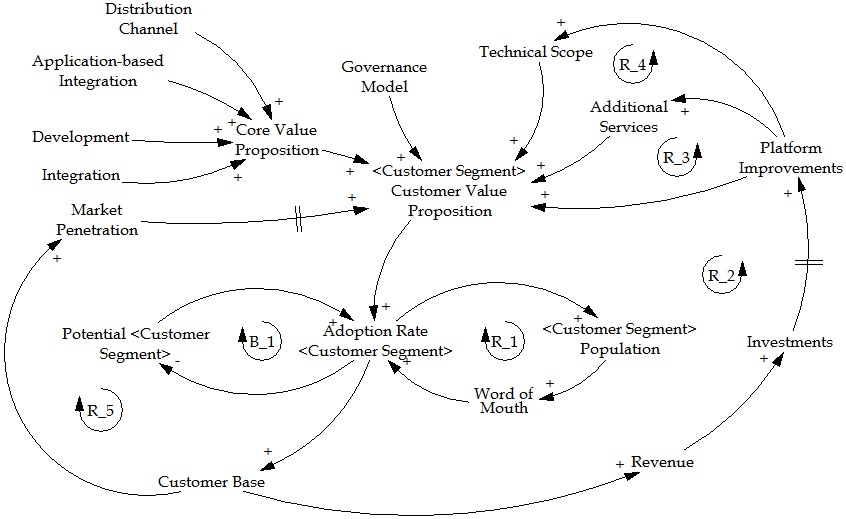
\includegraphics[width=\textwidth]{gfx/cld_customerSegment}
	\caption{Causal Loop Diagram -- Generic PaaS Customer Segment}
	\label{fig:cld_cs}
\end{figure}

In addition to the two above mentioned links to the adoption rate <customer segment>, the main link in the \ac{PaaS} domain is the influence link through the <customer segment> customer value proposition. As discussed earlier, the business model conceptualization proposed by \citet{Johnson2008} emphasizes to provide a dedicated \ac{CVP} for each customer segment to take the different customer needs explicitly into account. Thus, all five identified customer segments receive their own, dedicated \ac{CVP}. The relationship between the <customer segment> customer value proposition and the adoption rate <customer segment> is naturally a link with a positive polarity -- an increase in the <customer segment> customer value proposition will increase the adoption rate <customer segment> above what it would otherwise have been. During the evolution of the qualitative model, the aspect of the \ac{CVP} was discussed quite controversial. It was challenged, if it is necessary to model the \ac{CVP} quintuple, particularly for each customer segment. Finally, the discussion resulted in agreement that the consideration of five different \acp{CVP} is crucial to constitute the causal relationships in the \ac{PaaS} domain.

The <customer segment> customer value proposition itself is influenced sixfold -- through the (1) core value proposition, (2) governance model, (3) technical scope, (4) additional services, (5) market penetration, and (6) platform improvements. During the analysis of the 23 explorative case studies (especially in regards to the \ac{CVP}) as well as during the development of the classification scheme, a correlation between the core value proposition and the <customer segment> customer value proposition has been recognized. For the purpose of classifying \ac{PaaS} providers' it was argued that a provider is classified mainly by one core value proposition characteristic. However, in case of the qualitative model the core value proposition of a \ac{PaaS} provider is composed of all four identified core value proposition characteristics. The specific impact of the core value proposition onto the <customer segment> customer value proposition depends on the actual <customer segment> and needs to be further investigated for the transformation into a quantified model.

Moreover, the <customer segment> customer value proposition is influenced by two further classification criteria's -- namely the governance model and technical scope. Both criteria are mapped onto an ordinal scale, so it is straightforward to model the impact on the <customer segment> customer value proposition. An increase in the value of the technical scope or governance model will increase the <customer segment> customer value proposition above what it would otherwise have been. Also here the specific impact of both variables onto the <customer segment> customer value proposition depends on the actual <customer segment> and needs to be further investigated for the transformation into a quantified model. The two variables governance model and core value proposition (respectively its four influence variables) will remain constant, due to the fact that these variables are not influenced itself by any other variables.

Another point which was discussed during the 	evolution of this qualitative model was how to include the identified revenue streams into the model. Based on the lack of knowledge of user preferences concerning the revenue streams, these are excluded of the model because they cannot be modeled realistic. Further research is necessary to determine which revenue streams are preferred by the \ac{PaaS} stockholders. However, the analysis of the 23 explorative case studies revealed that nearly all \ac{PaaS} providers offer complementary products and especially services, for instance trainings, certifications, and consultancy services. Hence, it is inferred that these complements (henceforth referred to as additional services) influence the <customer segment> customer value proposition favorable. An increase in the value of the additional services variable will increase the value of the <customer segment> customer value proposition above what it would otherwise have been. Once again, the specific impact of the variable additional services onto the <customer segment> customer value proposition depends on the actual <customer segment> and needs to be further investigated for the transformation into a quantified model.

In the opposite direction, the adoption rate <customer segment> influences the variable customer base positive -- an increase in the adoption rate <customer segment> will increase the customer base above what it would otherwise have been. The impacts of the variable customer base are twofold. First, an increase in the variable customer base will increase the variable revenue above what it would otherwise have been. In return, an increase in the variable revenue will increase the value of the variable investments above what it would otherwise have been. Continuing, an increase in the variable investments will increase the variable platform improvements delayed above what it would otherwise have been. The variable platform improvements influences three above already mentioned variables -- <customer segment> customer value proposition, additional services, and technical scope -- and thus three further self-reinforcing feedback loops are identified (labeled as R\_2\footnote{R\_2: Customer Base -- Revenue -- Investments --- Platform Improvements -- <Customer Segment> Customer Value Proposition -- Adoption Rate <Customer Segment> -- Customer Base}, R\_3\footnote{R\_3: Customer Base -- Revenue -- Investments --- Platform Improvements -- Additional Services -- <Customer Segment> Customer Value Proposition -- Adoption Rate <Customer Segment> -- Customer Base}, and R\_4\footnote{R\_4: Customer Base -- Revenue -- Investments --- Platform Improvements -- Technical Scope -- <Customer Segment> Customer Value Proposition -- Adoption Rate <Customer Segment> -- Customer Base}). As already mentioned a couple of times above, the specific impact of the variable platform improvements onto the <customer segment> customer value proposition, additional services, and technical scope depends on the actual <customer segment> and needs to be further investigated for the transformation into a quantified model.

The second impact of the variable customer base concerns the variable market penetration. An increase in the variable customer base will increase the variable market penetration above what it would otherwise have been. Within the 23 explorative case studies it was remarkable that a company's brand image respectively the company's reputation was an important element of its \ac{CVP}. It is concluded that this issue will influence the <customer segment> customer value proposition, even though this impact will occur delayed. Hence, an increase in the variable market penetration will increase the variable <customer segment> customer value proposition delayed above what it would otherwise have been. The above described causal relationships constitute the fifth self-reinforcing feedback loop (labeled as R\_5\footnote{R\_5: Customer Base -- Market Penetration --- <Customer Segment> Customer Value Proposition -- Adoption Rate <Customer Segment> -- Customer Base}).

\section{Platform as a Service Customer Segment Interdependencies}\label{ch:cld:csi}

In this section the interdependencies between the in Chapter \ref{ch:sota} identified customer segments are discussed and depicted in Figure \ref{fig:cld_csi}. \citet[p. 33]{Cusumano2010} reasoned, that \textit{"the critical distinguishing feature of an industry platform and ecosystem is the creation of 'network effects'. These are positive feedback loops that can grow at geometrically increasing rates as adoption of the platform and the complements rise. The network effects can be very powerful \ldots~."} The in the previous section described self-reinforcing feedback look R\_1 represents a direct network effect or also known as same-side network effect. Gaming platforms are a well-known example of this network effect -- the more gamers are using a certain platform, the more valuable the platform becomes for other gamers. However, the direct network effects within the \ac{PaaS} domain are not considered as the crucial decisive factor. In contrast, indirect network effects are likely to be one of the main decisive factors. In general, an indirect network effect arises if there are cross-sided network effects in both directions (from A to B and vice versa). Once again gaming platforms are used as a common example: The platform value for gamers depends among other things on the number of games available for the platform. On the other side, those games are provided by game developers whose perceived platform value depends on the number of gamers using the platform. Frequently accompanied by such indirect network effects is the so called chicken-and-egg launch problem. 

Platform customers are characterized as upper \acp{SME} or large enterprises using the platform mainly for internal purposes. The introduction of a platform for these customers is most likely an extensive project which is often supported externally through \acp{SI}. Therefore, an increase in the platform customer population will increase the systems integrator population above what it would otherwise have been. Due to illustration reasons, the above described causal relationship as well as the corresponding depiction in Figure \ref{fig:cld_csi} is simplified. Actually an increase in the platform customer population will increase the systems integrator customer value proposition, which in turn will increase the adoption rate systems integrator, which finally will increase the systems integrator population. This simplification pattern applies also to the hereafter mentioned \ac{PaaS} customer segment dependencies. In the opposite direction, an increase in the systems integrator population will increase the platform customer population above what it would otherwise have been. Due to the fact that this causal relation is considered as weak, because no potential platform customer will adopt the platform solely if there is a large systems integrator population, it is shown dashed. However, even though this relationship is weak, a correlation can be noticed. Taken together the sixth self-reinforcing feedback loop has been found (labeled as R\_6\footnote{R\_6: Platform Customer Population -- Systems Integrator Population - - Platform Customer Population}). The platform customer population is further influenced by the variable platform modules\footnote{Platform modules are defined as \textit{"an add-on software subsystem that connects to the platform to add functionality to the platform"} \citep[p. 676]{Tiwana2010}, cf. Section \ref{ch:tf:paas:def}.}, although again with a weak impact.

\begin{figure}[tb]
	\centering
	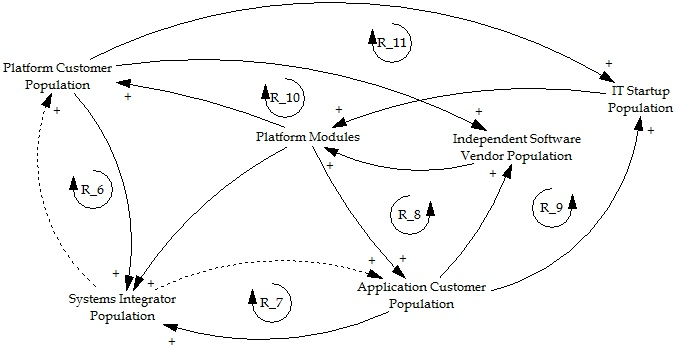
\includegraphics[width=\textwidth]{gfx/cld_customerSegmentInterdependencies}
	\caption{Causal Loop Diagram -- PaaS Customer Segment Interdependencies}
	\label{fig:cld_csi}
\end{figure}

A similar feedback loop can be identified between the systems integrator population and the application customer population. Also the introduction of platform modules is occasional supported through \acp{SI}. Therefore an increase in the application customer population will increase the systems integrator population above what it would otherwise have been. As with the platform customers, the application customer population is influenced by the systems integrator population, notwithstanding this causal connection is relatively weak. The above mentioned correlation builds the seventh self-reinforcing feedback loop (labeled as R\_7\footnote{R\_7: Systems Integrator Population - - Application Customer Population -- Systems Integrator Population}).

Platform modules -- applications, services, or add-ons -- are developed and provided by \ac{IT} startups and \acp{ISV} and thus an increase in the \ac{IT} startup population or independent software vendor population will increase the variable platform modules above what it would otherwise have been. The variable platform modules itself influences the application customer population positive -- an increase in the variable platform modules will increase the application customer population above what it would otherwise have been. And finally, the application customer population influences both platform module provider populations, an increase in the application customer population will increase the \ac{IT} startup population as well as independent software vendor population above what it would otherwise have been. Thereby the last two self-reinforcing feedback loops are closed (labeled as R\_8\footnote{R\_8: Application Customer Population -- \ac{IT} Startup Population -- Platform Modules -- Application Customer Population}  and R\_9\footnote{R\_9: Application Customer Population -- Independent Software Vendor Population -- Platform Modules -- Application Customer Population}).

\section{The Big Picture}\label{ch:cld:bp}

\begin{figure}[tb]
	\centering
	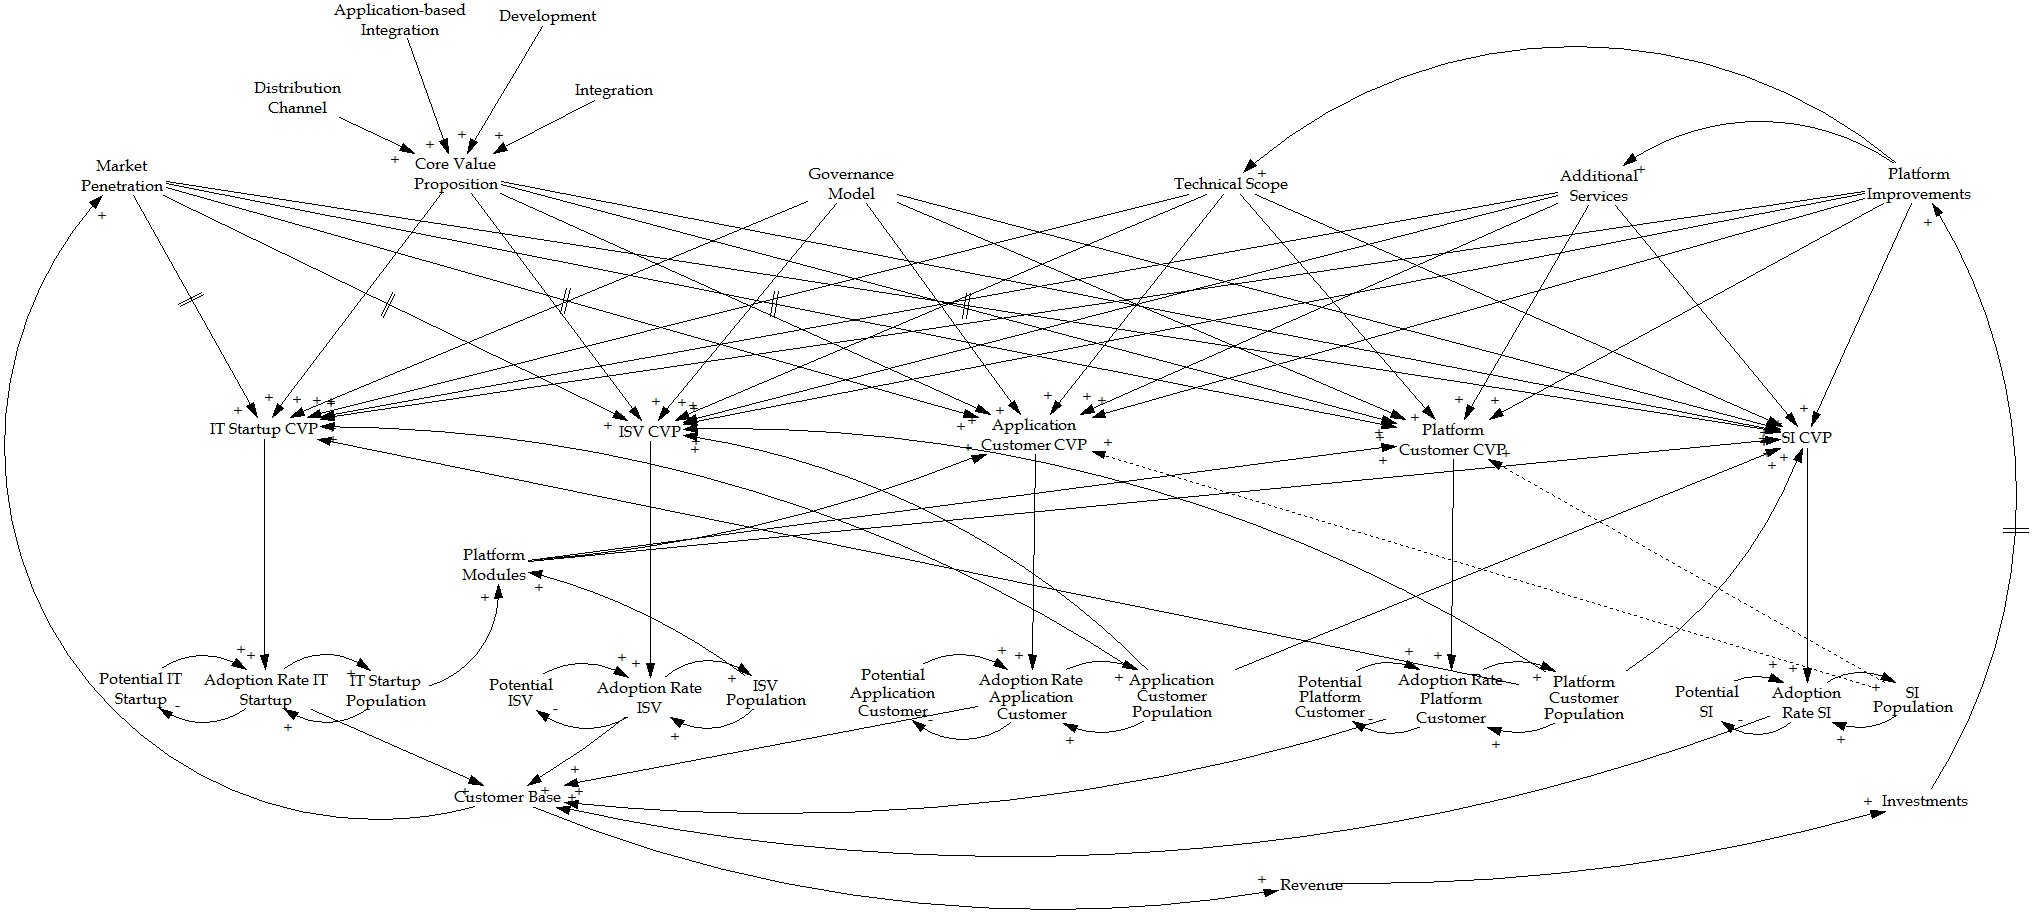
\includegraphics[height=0.95\textheight]{gfx/cld_bigPicture}
	\caption{Causal Loop Diagram -- The Big Picture}
	\label{fig:cld_bp}
\end{figure}

Finally, the overall qualitative model -- the big picture (cf. Figure \ref{fig:cld_bp}) -- based on the two above discussed sub-models can be illustrated. Within this model, the generic \ac{PaaS} customer segment sub-model exists five times -- corresponding to the five distinct customer segments. Moreover, also the \ac{PaaS} customer segment interdependencies sub-model is present in the overall model. However, in contrast to the \ac{PaaS} customer segment interdependencies sub-model, the therein simplified relationships are represented within the overall model in detail. In Section \ref{ch:cld:csi} the above mentioned simplification is briefly discussed.

All presented causal relationships within the overall model are already introduced in Section \ref{ch:cld:cs} as well as \ref{ch:cld:csi} and therefore not explained over again. In the first moment, the appearance of the big picture is possibly confusing, for instance through plenty of crossed links. Nevertheless with caution of the two in detail described sub-models and composition of the overall model, the structure and intention of this model should be clear.

As mentioned earlier, one important modeling aspect is to define suitable model boundaries. Previously already a couple of design decisions during the evolution of the qualitative model were mentioned and hereafter further challenges are discussed.

Even though in the model the aspect of revenue is considered basically (an increase in the customer base will increase the revenue above what it would otherwise have been and so forth, compare also the feedback loops R\_2, R\_3, and R\_4 within Figure \ref{fig:cld_cs}), the unarguable important aspect of costs is not considered at all. In order to do so, an uncountable number of criteria are necessary to model costs appropriate. For instance, the costs depend among other things from the deployment model, location, size of the company, and number of developers. The aspect of costs for the here discussed problem cannot be modeled sufficient in the available time frame and is therefore excluded from the model.

Another aspect which is considered, however in simplified terms, represents the market penetration. In the model an increase in the customer base will increase the market penetration above what it would otherwise have been and thereby influence the corresponding \ac{CVP} positive, through the company's brand image and company's reputation. The value of market penetration depends solely on the inherent model values, to be exact from the potential <customer segment>'s and <customer segment> populations values. Actually, the value of the market penetration depends also and decisive from the competition. The threat of new entrants and the rivalry among existing competitors \citep[pp. 80-82, 85-86]{Porter2008} are the most considerable forces here. However, in order to model the \ac{PaaS} market in a proper way various other model variables -- like own market share, competition market share, threat of new entrants, and overall market penetration -- and further assumptions are necessary. The attempt	 to add the whole \ac{PaaS} market to the model is rather like opening Pandora's box without increasing the model quality. This is why the \ac{PaaS} market in the overall model is simplified represented through the variable market penetration.

In the following Figure \ref{fig:cld_bp} the overall model -- the big picture -- is depicted: